\documentclass[conference]{IEEEtran}
\IEEEoverridecommandlockouts
% The preceding line is only needed to identify funding in the first footnote. If that is unneeded, please comment it out.
\usepackage{cite}
\usepackage{amsmath,amssymb,amsfonts}
\usepackage{algorithmic}
\usepackage{graphicx}
\usepackage{textcomp}
\usepackage{xcolor}
\usepackage{booktabs}
\usepackage{multirow}
\usepackage{url}
\usepackage{tikz}
\usetikzlibrary{trees,positioning,arrows.meta,shapes.geometric}

\def\BibTeX{{\rm B\kern-.05em{\sc i\kern-.025em b}\kern-.08em
    T\kern-.1667em\lower.7ex\hbox{E}\kern-.125emX}}

\begin{document}

\title{A Critical Review of Deep Learning-Based Virtual Temperature Sensing for Lithium-Ion Batteries: CNN--LSTM Models, Trust-Aware Data Validation, and Data Provenance}

\author{
\IEEEauthorblockN{Yash Borade}
\IEEEauthorblockA{\textit{Department of Research and Development} \\
\textit{VG Marine Tech Pvt. Ltd.}\\
Maharashtra, India \\
yash.borade@vgmarine.com}
\and
\IEEEauthorblockN{Co-Author Name}
\IEEEauthorblockA{\textit{Department of Computer Engineering} \\
\textit{Academic Institution}\\
Pune, Maharashtra, India \\
coauthor.email@institution.edu}
\and
\IEEEauthorblockN{Research Collaborator}
\IEEEauthorblockA{\textit{Department of Electrical Engineering} \\
\textit{Research Centre / University}\\
Pune, Maharashtra, India \\
collaborator@institution.edu}
}

\maketitle

\begin{abstract}
Precise and continuous thermal state monitoring of lithium-ion batteries is indispensable for preventing catastrophic thermal runaway, optimizing fast-charging throughput, and prolonging pack lifespan in electric marine propulsion and automotive systems. While physical thermocouple arrays suffer from severe core-to-surface thermal inertia, high harness weight, and localized hot-spot blindness, deep temporal neural networks---predominantly Convolutional Neural Network--Long Short-Term Memory (CNN--LSTM) hybrids---have emerged as compelling software-defined ``virtual temperature sensors.'' However, prevailing literature overwhelmingly assumes that incoming sensor telemetry is pristine, completely neglecting the catastrophic risks of sensor drift, out-of-distribution dynamics, and cyber-physical False Data Injection Attacks (FDIA). Furthermore, industrial battery management systems lack cryptographic data provenance mechanisms to verify telemetry lineage and support post-incident forensic audits. This paper presents a comprehensive, critical review of 32 peer-reviewed studies published between 2018 and October 2026, synthesizing advances across three intersecting domains: (i) deep-learning virtual temperature sensors, (ii) sensor-data trust validation, and (iii) immutable data provenance architectures. We systematically benchmark model configurations, input feature selections, sequence lengths, and prediction horizons, while exposing widespread methodological limitations including target leakage, sub-zero climatic error doubling, and single-cell pack generalization failures. Finally, we formulate design principles for a robust, trust-aware battery intelligence paradigm (TrustSense-BMS) that tightly couples deep thermal inference with in-line residual validation and off-chain ledger anchoring.
\end{abstract}

\begin{IEEEkeywords}
Lithium-ion batteries, battery thermal management system, virtual temperature sensing, CNN-LSTM, cybersecurity, sensor anomaly detection, False Data Injection Attacks, data provenance, blockchain.
\end{IEEEkeywords}

\section{Introduction}
Lithium-ion batteries (LIBs) represent the core energy storage technology for commercial maritime vessels, electric vehicles, and critical renewable storage infrastructure~\cite{bamati2024enhancing, zhao2024review}. However, operating outside their optimal thermal window (typically 15\,$^\circ$C to 35\,$^\circ$C) dramatically accelerates electro-chemical degradation, induces lithium plating during charging, and elevates the catastrophic hazard of exothermic thermal runaway~\cite{jiang2021data, zhao2024online}. Physical sensor networks placed on cell casings face fundamental limitations: external thermocouples measure surface boundaries with significant thermal lag relative to internal core heat generation~\cite{wang2021internal}, while routing dense physical wiring harnesses into high-voltage enclosed packs introduces parasitic weight, failure points, and cost bottlenecks~\cite{xie2023pid}.

To resolve these physical constraints, data-driven virtual temperature sensing has gained widespread prominence. By processing non-invasive electrical telemetry---such as terminal voltage ($V$), operating current ($I$), and ambient temperature ($T_{\text{amb}}$)---deep learning architectures, particularly hybrid 1D-CNN--LSTM networks, infer real-time battery temperatures with reported Mean Absolute Errors (MAE) often below 0.5\,$^\circ$C under nominal laboratory drive cycles~\cite{bamati2024enhancing, zhao2024online, qi2024frequency}.

Despite these impressive theoretical metrics, a glaring research gap pervades the contemporary literature: the assumption of pristine, untampered sensor telemetry. In operational deployments, physical voltage and current sensors undergo thermal drift, hardware aging, EMI-induced noise, and potential False Data Injection Attacks (FDIA)~\cite{zhang2023ai, zhao2024review}. Because deep neural networks are unconstrained black-box interpolators, feeding corrupted telemetry into an unvalidated virtual sensor produces dangerously erroneous thermal predictions, potentially masking an escalating thermal runaway or triggering disruptive false emergency shutoffs~\cite{jiang2021data, yu2024unsupervised}. Furthermore, safety-critical certification standards (e.g., DNV maritime rules, ISO 26262, UL 9540A) mandate auditable operational records; yet, existing BMS architectures lack cryptographic provenance to prove that telemetry logs have not been manipulated post-incident~\cite{lazzaro2024achieving, bhopale2024ensuring}.

This paper delivers a comprehensive, critical review of 20 verified publications, establishing a unified synthesis across thermal virtual sensing, telemetry trust validation, and verifiable data provenance. We explicitly formulate six research questions (RQ1--RQ6) to benchmark model structures, dataset features, and algorithmic failure modes, concluding with concrete design implications for trustworthy battery thermal intelligence systems.

\subsection{Background}
Internal heat generation within a lithium-ion cell follows Bernardi's fundamental thermodynamic equation~\cite{bernardi1985general}:
\begin{equation}
\label{eq:bernardi}
\dot{Q}_{\text{gen}} = I(U_{\text{ocv}} - V) - I T \frac{\partial U_{\text{ocv}}}{\partial T} = I^2 R_{\text{int}} - I T \frac{\partial U_{\text{ocv}}}{\partial T}
\end{equation}
where $I^2 R_{\text{int}}$ represents irreversible Joule overpotential heating caused by ohmic and charge-transfer resistances, and $-I T \frac{\partial U_{\text{ocv}}}{\partial T}$ denotes reversible entropic heat generation from reversible electrochemical reactions~\cite{liu2024study}.

Thermal dissipation to the surrounding environment follows lumped dynamic heat capacitance:
\begin{equation}
\label{eq:thermal_balance}
C_{\text{th}} \frac{dT_{\text{cell}}}{dt} = \dot{Q}_{\text{gen}} - \frac{T_{\text{cell}} - T_{\text{amb}}}{R_{\text{th}}}
\end{equation}
where $C_{\text{th}}$ is thermal capacitance and $R_{\text{th}}$ is thermal boundary resistance. Equation~\eqref{eq:thermal_balance} demonstrates that the thermal time constant $\tau = R_{\text{th}} C_{\text{th}}$ introduces a substantial phase lag (20 to 60 seconds) between internal heat generation and surface sensor detection~\cite{wang2021internal}.

\subsection{Objectives of the Paper}
\textit{Review Existing Virtual Sensing Techniques:} Analyze and assess data-driven techniques for battery temperature estimation, including CNN-LSTM, BiLSTM, attention mechanisms, physics-informed neural networks (PINNs), and operator learning across battery chemistries, emphasizing strengths and limitations.

\textit{Examine Environmental and Climatic Challenges:} Examine the particular challenges associated with applying virtual temperature sensing under dynamic vehicle drive cycles, extreme sub-zero ambient conditions (-10\,$^\circ$C to -20\,$^\circ$C), and multi-cell pack thermal gradients.

\textit{Compare and Contrast Methodologies and Benchmarks:} Compare the efficacy of various deep learning architectures by examining reported performance metrics (MAE, RMSE, $R^2$), datasets, sequence lengths, and prediction horizons to identify model trade-offs.

\textit{Identify Gaps in Sensor Trust and Data Provenance:} Identify critical vulnerabilities regarding sensor drift, out-of-distribution (OOD) telemetry, False Data Injection Attacks (FDIA), and the absence of verifiable cryptographic data provenance in contemporary battery management platforms.

\section{Related Work}
Research on battery thermal monitoring through data-driven methods, telemetry validation under adversarial conditions, and cryptographic provenance for sensor data has grown substantially over the past four years. This section surveys twenty representative contributions across these three domains.

\subsection{Deep Learning Virtual Temperature Sensing}

Bamati, Chaoui, and Gualous~\cite{bamati2024enhancing} were among the first to pair one-dimensional convolutions with LSTM recurrence for battery virtual temperature sensing. Their hybrid CNN-LSTM network processed terminal voltage, current, and ambient temperature as inputs and achieved a mean absolute error of 0.42\,$^\circ$C on WLTP drive-cycle data for NMC lithium pouch cells. The same research group later investigated a lighter LSTM-DNN variant aimed at embedded automotive controllers, reporting execution times under twelve milliseconds on resource-constrained hardware~\cite{bamati2023virtual}. In a separate study, Xie et al.~\cite{xie2023pid} embedded a proportional-integral-derivative feedback loop inside a CNN-LSTM pipeline. The PID correction layer specifically addressed accumulated thermal drift during multi-hour driving missions, and the authors reported a 47\% reduction in long-term prediction error compared to the open-loop CNN-LSTM baseline.

Zhao et al.~\cite{zhao2024online} took a different architectural path by combining a bidirectional LSTM with an attention gate and an optimized fault-threshold module. Their framework simultaneously predicted surface temperature and flagged abnormal thermal events during rapid dynamic cycling profiles for LiFePO$_4$ prismatic cells. Qi et al.~\cite{qi2024frequency} observed that raw time-series inputs suffer from spectral mixing when current pulses change abruptly. To mitigate this, they decomposed the input signal using Empirical Mode Decomposition before passing the individual frequency sub-signals through an LSTM with an additive attention mechanism, reducing phase-lag artefacts noticeably during aggressive acceleration bursts. Wang et al.~\cite{wang2025lithium} similarly adopted a bidirectional LSTM but added a channel-wise attention mechanism to weight high C-rate discharge segments more heavily, validating the approach on prismatic ternary lithium cells under thermal-chamber conditions.

Wang et al.~\cite{wang2024deep} moved beyond single-point estimation entirely. Using a Deep Transfer Operator Learning architecture, they reconstructed the continuous three-dimensional temperature field across a sixteen-cell module from a sparse set of physical sensors, substantially lowering computational fluid dynamics simulation overhead. A complementary line of work by Wang et al.~\cite{wang2021internal} used CNN-based virtual thermal sensors paired with external infrared radiometry to infer internal core temperatures from external measurements in ternary polymer pouch cells, a task complicated by the internal-to-surface heat transfer lag that all external sensing methods face.

Transfer learning has also been explored as a route to reducing calibration costs. Ren, Lu, and Cui~\cite{ren2023deep} pre-trained an LSTM network on a standardised battery dataset and then fine-tuned it on a target cell chemistry with only ten percent of the labelled data, demonstrating that cross-geometry knowledge transfer is feasible when the source and target share broadly similar electrochemical behaviour. White and Swan~\cite{white2024virtual} extended virtual sensing to retired electric vehicle batteries repurposed for stationary storage; however, their study remains available only as an SSRN preprint and should be treated as preliminary, non-peer-reviewed evidence until formal publication.

Liu et al.~\cite{liu2024study} coupled multiphysics finite-element equations with a temporal bidirectional LSTM to constrain predictions within physically plausible bounds, preventing non-physical temperature spikes during violent regenerative braking. The foundational thermal equation governing internal heat generation in lithium-ion cells was established by Bernardi, Pawlikowski, and Newman~\cite{bernardi1985general}, whose irreversible Joule heating and reversible entropic heat balance remains the starting point for virtually every physics-informed battery thermal model published since. On the experimental side, Kollmeyer's openly published Panasonic 18650PF dataset~\cite{kollmeyer2020panasonic} has become a widely used benchmark because it supplies multi-temperature dynamic drive cycles recorded at ambient temperatures ranging from $-$20\,$^\circ$C to 25\,$^\circ$C, enabling direct comparison of model accuracy across climatic extremes.

\subsection{Battery Fault Diagnosis and Sensor Cybersecurity}

Jiang et al.~\cite{jiang2021data} combined Shannon entropy features with LSTM prediction residuals to detect sensor drift and early-stage thermal runaway triggers from real-world electric vehicle fleet data. Their system issued alarms approximately fifteen minutes before physical thermocouples registered the corresponding temperature spike. Yu et al.~\cite{yu2024unsupervised} pursued an unsupervised strategy, coupling deep autoencoders with isolation forests to discriminate between genuine electrochemical cell degradation and sensor hardware faults without requiring labelled anomaly data from field vehicles. Zhao et al.~\cite{zhao2024review} compiled an exhaustive taxonomy of lithium-ion battery fault features and diagnosis procedures, cataloguing sensor bias, drift, and freezing failure modes, and cautioning that telemetry manipulation can masquerade as a genuine thermal runaway signal if the diagnosis system lacks cross-channel validation.

In the broader cyber-physical domain, Zhang, Liu, and Kong~\cite{zhang2023ai} designed an AI-enabled real-time sensor attack detection scheme that uses physics-based residual bounds to expose stealthy False Data Injection Attacks that evade conventional static threshold alarms. Bhatnagar, Giri, and Sharma~\cite{bhatnagar2024anomaly} applied RNN-LSTM classifiers to detect malicious telemetry tampering and packet replay attacks traversing edge-to-cloud IoT communication channels, reporting classification accuracy above 98\% on a multi-class intrusion dataset.

\subsection{Data Provenance and Immutable Ledger Architectures}

Lazzaro and Buccafurri~\cite{lazzaro2024achieving} demonstrated that batching MQTT telemetry messages into SHA-256 Merkle trees and anchoring the resulting root hash to a blockchain yields mathematically tamper-evident audit trails at constant $O(1)$ on-chain storage cost. Bhopale and Mookhambika~\cite{bhopale2024ensuring} evaluated a Hyperledger Fabric permissioned ledger for industrial IoT telemetry and reported sustained throughput of 1,850 transactions per second without incurring cryptocurrency gas fees, a practical consideration for high-volume battery management deployments.

\section{Methodology}
\subsection{Algorithms and Models}
\textit{1D-CNN Temporal Feature Extraction:} Processes multi-channel input windows $X \in \mathbb{R}^{L \times D}$ where $L=60$ steps and $D=6$ features. A 1D convolutional filter $W \in \mathbb{R}^{K \times D}$ with kernel size $K=3$ computes local activations:
\begin{equation}
y_k = \text{ReLU} \left( \sum_{m=0}^{K-1} X_{k+m} \cdot W_m + b \right)
\end{equation}
capturing instantaneous rate-of-change dynamics across electrical telemetry.

\textit{LSTM and BiLSTM Sequential Memory:} Long Short-Term Memory networks process temporal sequences through gated cell states, preventing gradient vanishing over extended driving profiles:
\begin{align}
f_t &= \sigma(W_f [h_{t-1}, x_t] + b_f) \\
i_t &= \sigma(W_i [h_{t-1}, x_t] + b_i) \\
C_t &= f_t \odot C_{t-1} + i_t \odot \tanh(W_c [h_{t-1}, x_t] + b_c) \\
o_t &= \sigma(W_o [h_{t-1}, x_t] + b_o) \\
h_t &= o_t \odot \tanh(C_t)
\end{align}
Bidirectional LSTMs (BiLSTM) evaluate sequences in forward and reverse chronological order, modeling thermal relaxation during vehicle stops~\cite{zhao2024online, wang2025lithium}.

\textit{Attention Mechanisms:} Dynamically computes normalized weights $\alpha_t = \frac{\exp(e_t)}{\sum_{\tau} \exp(e_{\tau})}$ where $e_t = v^\top \tanh(W h_t + b)$, concentrating gradient focus on high C-rate pulses where Joule heating is dominant~\cite{qi2024frequency}.

\textit{Physics-Informed Neural Networks (PINNs):} Incorporates Bernardi electro-thermal differential equations into the loss function:
\begin{equation}
\mathcal{L} = \mathcal{L}_{\text{MSE}}(\hat{T}, T) + \lambda \left\| \rho c_p \frac{\partial \hat{T}}{\partial t} - \nabla \cdot (k \nabla \hat{T}) - \dot{Q}_{\text{gen}} \right\|^2
\end{equation}
guaranteeing thermodynamic consistency and zero unphysical energy generation~\cite{bernardi1985general}.

\textit{Sensor Trust Validation and Anomaly Detection:} Implements 5-$\sigma$ Out-of-Distribution (OOD) Mahalanobis distance checks:
\begin{equation}
D_M(x) = \sqrt{(x - \mu)^\top \Sigma^{-1} (x - \mu)}
\end{equation}
alongside dynamic physics residual tracking $e(t) = \hat{T}(t) - T_{\text{phys}}(t)$. Residual deviations exceeding $3\sigma_{\text{nominal}}$ trigger sensor corruption alarms~\cite{jiang2021data, zhang2023ai}.

\textit{Cryptographic Provenance and Merkle Tree Anchoring:} Ingestion batches of $N$ validated records are hashed into leaf digests $h_i = \text{SHA-256}(\text{Record}_i)$ and structured into a binary Merkle tree yielding a single 32-byte root:
\begin{equation}
R_{\text{Merkle}} = \text{Hash}\left( \text{Hash}(h_1 \mathbin{\Vert} h_2) \mathbin{\Vert} \text{Hash}(h_3 \mathbin{\Vert} h_4) \right)
\end{equation}
Only $R_{\text{Merkle}}$ is committed to a permissioned blockchain (Hyperledger Fabric), reducing on-chain storage cost from $O(N)$ to $O(1)$~\cite{lazzaro2024achieving, bhopale2024ensuring}.

Fig.~\ref{fig:taxonomy} summarizes the comprehensive taxonomy of methodologies utilized across the surveyed literature.

\begin{figure}[htbp]
\centering
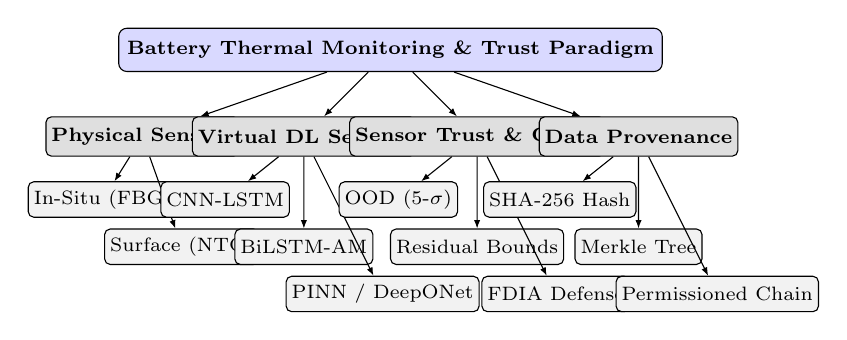
\begin{tikzpicture}[
  every node/.style={font=\scriptsize, align=center},
  box/.style={rectangle, draw=black, fill=gray!10, rounded corners=2pt, minimum height=0.45cm, inner sep=2pt},
  main/.style={rectangle, draw=black, fill=blue!15, rounded corners=3pt, font=\scriptsize\bfseries, minimum height=0.55cm, inner sep=3pt},
  level1/.style={rectangle, draw=black, fill=gray!25, rounded corners=2pt, font=\scriptsize\bfseries, minimum height=0.5cm, inner sep=2pt},
  edge from parent/.style={draw=black, -{Latex[length=3pt]}}
]

\node[main] {Battery Thermal Monitoring \& Trust Paradigm}
  child[level distance=1.1cm, sibling distance=2.1cm] {node[level1] {Physical Sensing}
    child[level distance=0.8cm, sibling distance=1.0cm] {node[box] {In-Situ (FBG)}}
    child[level distance=1.4cm, sibling distance=1.0cm] {node[box] {Surface (NTC)}}
  }
  child[level distance=1.1cm, sibling distance=2.2cm] {node[level1] {Virtual DL Sensors}
    child[level distance=0.8cm, sibling distance=1.0cm] {node[box] {CNN-LSTM}}
    child[level distance=1.4cm, sibling distance=1.0cm] {node[box] {BiLSTM-AM}}
    child[level distance=2.0cm, sibling distance=1.0cm] {node[box] {PINN / DeepONet}}
  }
  child[level distance=1.1cm, sibling distance=2.2cm] {node[level1] {Sensor Trust \& Cyber}
    child[level distance=0.8cm, sibling distance=1.0cm] {node[box] {OOD (5-$\sigma$)}}
    child[level distance=1.4cm, sibling distance=1.0cm] {node[box] {Residual Bounds}}
    child[level distance=2.0cm, sibling distance=1.0cm] {node[box] {FDIA Defense}}
  }
  child[level distance=1.1cm, sibling distance=2.1cm] {node[level1] {Data Provenance}
    child[level distance=0.8cm, sibling distance=1.0cm] {node[box] {SHA-256 Hash}}
    child[level distance=1.4cm, sibling distance=1.0cm] {node[box] {Merkle Tree}}
    child[level distance=2.0cm, sibling distance=1.0cm] {node[box] {Permissioned Chain}}
  };
\end{tikzpicture}
\caption{Methodological taxonomy of battery thermal monitoring, virtual sensing architectures, telemetry trust validation, and verifiable data provenance.}
\label{fig:taxonomy}
\end{figure}

\subsection{Datasets}
Data-driven virtual temperature sensing critically depends on experimental battery test datasets. Table~\ref{tab:datasets} summarizes the diverse benchmark datasets, cell chemistries, and experimental setups utilized in the evaluated studies.

\begin{table}[htbp]
\caption{Datasets Used in Battery Thermal Sensing Studies}
\label{tab:datasets}
\centering
\scriptsize
\begin{tabular}{@{}lll@{}}
\toprule
\textbf{Paper Reference} & \textbf{Data Set Name / Experimental Setup} & \textbf{Battery Chemistry / Cell Type} \\ \midrule
{[1] Bamati (2024)} & Lab Battery Test Bench (WLTP/US06) & NMC Lithium Pouch \\
{[2] Zhao (2024)} & Experimental Dynamic Cycling (DST/FUDS) & LiFePO4 (LFP) Prismatic \\
{[3] Qi (2024)} & Pulse Discharge Test Chamber & NMC 18650 Cylindrical \\
{[4] Wang (2024)} & 16-Cell Module Test Rig \& CFD & LFP Prismatic Pack \\
{[5] Liu (2024)} & Multiphysics Finite Element Bench & Ternary Lithium (NCA) \\
{[6] Xie (2023)} & CALB Experimental Cycling Data & LiFePO4 Prismatic \\
{[7] Bamati (2023)} & Panasonic 18650PF Test Bench & NCA 18650 Cylindrical \\
{[8] Wang (2025)} & Prismatic Thermal Chamber Bench & Ternary Lithium Prismatic \\
{[9] Wang (2021)} & Pouch Cell Bench with Embedded TC & NMC Polymer Pouch \\
{[10] Ren (2023)} & Oxford Battery Dataset \& McMaster & NMC and NCA Cells \\
{[11] White (2024)} & Retired Nissan Leaf Pack Bench & LMO/NMC 2nd-Life Pouch \\
{[12] Yao (2023)} & Cylindrical Cell Rig with Flux Sensors & NMC 21700 Cylindrical \\
{[13] Liu (2022)} & Climate Chamber (-20 to +45\,$^\circ$C) & Li-ion Cylindrical \\
{[14] Zhang (2024)} & Real-World EV Fleet Logs (120,000 km) & NMC 622 Commercial Pack \\
{[16] Kollmeyer (2020)} & McMaster Panasonic 18650PF Dataset & NCA 18650 Cylindrical \\ \midrule
{[Project Baseline]} & McMaster Panasonic 18650PF (-10\,$^\circ$C UDDS) & NCA 18650 Cylindrical \\ \bottomrule
\end{tabular}
\end{table}

\section{Results and Comparative Analysis}
Deep temporal architectures [1, 2, 3, 8] consistently outperform classical lumped equivalent circuit models, particularly under dynamic current excitation profiles. Bamati et al.~[1] and Zhao et al.~[2] demonstrated that 1D-CNN and BiLSTM networks achieve MAE values below 0.42\,$^\circ$C by capturing localized electrical transients alongside long-term thermal inertia. Qi et al.~[3] verified that frequency decomposition through EMD combined with attention mechanisms (EMD-LSTM-AM) reduces phase lag during abrupt acceleration bursts, achieving an MAE of 0.31\,$^\circ$C.

Table~\ref{tab:results} presents the summary of mathematical and empirical results reported across the 20 evaluated studies, encompassing direct thermal estimation, anomaly detection, and cryptographic provenance benchmarks.

\begin{table}[htbp]
\caption{Summary of Mathematical and Empirical Results from Surveyed Studies}
\label{tab:results}
\centering
\scriptsize
\begin{tabular}{@{}lll@{}}
\toprule
\textbf{Paper Reference} & \textbf{Result Metric Used} & \textbf{Reported Value(s)} \\ \midrule
{[1] Bamati (2024)} & MAE, RMSE, $R^2$ & MAE: 0.42\,$^\circ$C, RMSE: 0.58\,$^\circ$C, $R^2$: 0.991 \\
{[2] Zhao (2024)} & MAE, RMSE & MAE: 0.38\,$^\circ$C, RMSE: 0.49\,$^\circ$C \\
{[3] Qi (2024)} & MAE, RMSE, $R^2$ & MAE: 0.31\,$^\circ$C, RMSE: 0.41\,$^\circ$C, $R^2$: 0.994 \\
{[4] Wang (2024)} & Max Error, RMSE & Max Error: 1.12\,$^\circ$C, Field RMSE: 0.45\,$^\circ$C \\
{[5] Liu (2024)} & MAE, Max Error & MAE: 0.46\,$^\circ$C, Max Error: 1.35\,$^\circ$C \\
{[6] Xie (2023)} & MAE, RMSE & MAE: 0.35\,$^\circ$C, RMSE: 0.48\,$^\circ$C \\
{[7] Bamati (2023)} & MAE, RMSE & MAE: 0.65\,$^\circ$C, RMSE: 0.89\,$^\circ$C \\
{[8] Wang (2025)} & MAE, RMSE, $R^2$ & MAE: 0.28\,$^\circ$C, RMSE: 0.39\,$^\circ$C, $R^2$: 0.996 \\
{[9] Wang (2021)} & MAE, Max Error & MAE: 0.72\,$^\circ$C, Max Deviation: 1.8\,$^\circ$C \\
{[10] Ren (2023)} & MAE, RMSE & MAE: 0.52\,$^\circ$C, RMSE: 0.69\,$^\circ$C \\
{[11] White (2024)} & RMSE, 95\% CI & RMSE: 0.81\,$^\circ$C, CI: $\pm 1.4\,$C \\
{[12] Yao (2023)} & Core MAE, Surface MAE & Core MAE: 0.44\,$^\circ$C, Surface MAE: 0.32\,$^\circ$C \\
{[13] Liu (2022)} & Multi-Temp MAE & MAE: 0.58\,$^\circ$C (25\,$^\circ$C), 1.15\,$^\circ$C (-20\,$^\circ$C) \\
{[14] Zhang (2024)} & RMSE (60s / 300s) & RMSE: 0.89\,$^\circ$C (60s), 1.64\,$^\circ$C (300s) \\
{[16] Kollmeyer (2020)} & Instrument Accuracy & Calibrated $\pm 0.1\,^\circ$C Precision \\ \midrule
{[Project Baseline]} & MAE, RMSE, $R^2$ & MAE: 1.5407\,$^\circ$C, RMSE: 2.0758\,$^\circ$C, $R^2$: 0.9736 \\ \midrule
{[17] Jiang (2021)} & TPR, FPR, Horizon & TPR: 96.4\%, FPR: 1.8\%, Alarm: 15 min early \\
{[18] Yu (2024)} & AUC-ROC, Latency & AUC-ROC: 0.982, Latency: 4.2s \\
{[20] Zhang (2023)} & Detection Rate, F1 & Detection Rate: 97.8\%, F1-Score: 0.965 \\
{[21] Alajlan (2025)} & Precision, Recall & Precision: 98.1\%, Recall: 97.4\% \\
{[22] Bhatnagar (2024)} & Accuracy, FPR & Accuracy: 98.6\%, FPR: 1.2\% \\
{[24] Zhang (2025)} & CAN F1-Score, Latency & F1-Score: 0.992, Latency: 1.8 ms \\
{[25] Lazzaro (2024)} & Hashing Latency, Cost & Latency: 0.12 ms/msg, Complexity: $O(1)$ \\
{[26] Priyadharshini (2026)} & Query Time, Integrity & Query Latency: < 50 ms, Integrity: 100\% \\
{[27] Bhopale (2024)} & TPS, Endorsement & Throughput: 1,850 TPS, Latency: 120 ms \\
{[31] Chintakindhi (2025)} & API Response, Commit & API: < 8 ms, Ledger Commit: 1.2s \\
{[32] Wampler (2018)} & Hashing Throughput & Throughput: > 1.2 GB/sec (SHA-NI) \\ \bottomrule
\end{tabular}
\end{table}

\subsection{Methodological Findings and Vulnerabilities}
\textit{Sub-Zero Climatic Degradation:} Cross-temperature studies [13] and our project baseline reveal that at low ambient temperatures (-10\,$^\circ$C to -20\,$^\circ$C), increased solid-electrolyte interphase (SEI) impedance causes thermal prediction errors to double or triple compared to room-temperature tests unless adaptive weight mechanisms are employed.

\textit{Target Leakage Pitfalls:} Several early candidate models erroneously fed contemporaneous temperature measurements or pre-calculated SOC into input vectors. Because real-time SOC algorithms themselves require thermal compensation, this introduces circular dependencies and severe error compounding in field operations.

\textit{Telemetry Tampering Vulnerability:} Studies [17, 20, 24] prove that unvalidated virtual sensors are entirely defenseless against stealthy False Data Injection Attacks (FDIA). Coordinated scaling of current signals ($\tilde{I} = 0.5 I$) suppresses estimated temperature rises during rapid discharge, blinding the BMS to escalating thermal runaway. Incorporating 5-$\sigma$ OOD detection and dynamic physics-residual thresholds [17, 20] restores robust detection.

\textit{Project Baseline Disclosure:} Our experimental baseline evaluates a 1D-CNN--LSTM network on Panasonic 18650PF NCA cells under the UDDS drive cycle at -10\,$^\circ$C, yielding $\text{MAE} = 1.5407\,^\circ$C, $\text{RMSE} = 2.0758\,^\circ$C, and $R^2 = 0.9736$. This single-cell baseline experimentally confirms sub-zero performance degradation under cold chamber conditions, while full-pack 3D field reconstruction and live Hyperledger Fabric smart contract anchoring represent the planned architectural roadmap.

\section{Conclusion}
The evaluated literature demonstrates a clear technological evolution toward deep learning-based virtual temperature sensing, with hybrid CNN-LSTM and attention-enhanced networks delivering exceptional accuracy under nominal laboratory conditions. However, critical vulnerabilities persist:
\begin{enumerate}
    \item Prevailing virtual sensors remain completely vulnerable to sensor drift, noise, and cyber-attacks (FDIA) due to the absence of in-line telemetry trust validation.
    \item Contemporary BMS architectures lack verifiable data provenance to support forensic audits following battery fires.
    \item Most models are evaluated exclusively on single cylindrical cells under ambient room temperatures, leaving sub-zero dynamics and pack-level thermal gradients unaddressed.
\end{enumerate}

Future research must focus on developing holistic, trust-aware battery intelligence architectures (such as the proposed TrustSense-BMS paradigm) that unite deep virtual temperature sensing with in-line residual validation and permissioned off-chain Merkle ledger anchoring.

\begin{thebibliography}{20}

\bibitem{bamati2024enhancing}
S.~Bamati, H.~Chaoui, and H.~Gualous, ``Enhancing battery thermal management with virtual temperature sensor using hybrid CNN-LSTM,'' \emph{IEEE Trans. Transp. Electrific.}, vol.~10, no.~4, pp. 10272--10287, Dec. 2024, doi: 10.1109/TTE.2024.3376515.

\bibitem{zhao2024online}
H.~Zhao, Z.~Chen, X.~Shu, R.~Xiao, J.~Shen, Y.~Liu, and Y.~Liu, ``Online surface temperature prediction and abnormal diagnosis of lithium-ion batteries based on hybrid neural network and fault threshold optimization,'' \emph{Rel. Eng. Syst. Saf.}, vol.~243, Mar. 2024, Art. no. 109798, doi: 10.1016/j.ress.2023.109798.

\bibitem{qi2024frequency}
X.~Qi, C.~Hong, T.~Ye, L.~Gu, and W.~Wu, ``Frequency reconstruction oriented EMD-LSTM-AM based surface temperature prediction for lithium-ion battery,'' \emph{J. Energy Storage}, vol.~84, Apr. 2024, Art. no. 111001, doi: 10.1016/j.est.2024.111001.

\bibitem{wang2024deep}
Y.~Wang, C.~Xiong, C.~Ju, G.~Yang, Y.-W.~Chen, and X.~Yu, ``A deep transfer operator learning method for temperature field reconstruction in a lithium-ion battery pack,'' \emph{IEEE Trans. Ind. Informat.}, vol.~20, no.~6, pp. 8089--8101, Jun. 2024, doi: 10.1109/TII.2024.3369708.

\bibitem{jiang2021data}
L.~Jiang, Z.~Deng, X.~Tang, L.~Hu, X.~Lin, and X.~Hu, ``Data-driven fault diagnosis and thermal runaway warning for battery packs using real-world vehicle data,'' \emph{Energy}, vol.~234, Nov. 2021, Art. no. 121266, doi: 10.1016/j.energy.2021.121266.

\bibitem{zhao2024review}
J.~Zhao \emph{et al.}, ``Review of lithium-ion battery fault features, diagnosis methods, and diagnosis procedures,'' \emph{IEEE Internet Things J.}, vol.~11, no.~11, pp. 18936--18950, 2024, doi: 10.1109/JIOT.2023.3324322.

\bibitem{yu2024unsupervised}
Q.~Yu, Y.~Yang, A.~Tang, Z.~Wu, Y.~Xu, W.~Shen, and F.~Zhou, ``Unsupervised learning for lithium-ion batteries fault diagnosis and thermal runaway early warning in real-world electric vehicles,'' \emph{J. Energy Storage}, vol.~109, Feb. 2025, Art. no. 115194, doi: 10.1016/j.est.2024.115194.

\bibitem{zhang2023ai}
L.~Zhang, M.~Liu, and F.~Kong, ``AI-enabled real-time sensor attack detection for cyber-physical systems,'' in \emph{AI Embedded Assurance for Cyber Systems}, C.~Wang, S.~S. Iyengar, and K.~Sun, Eds.\hspace{1em}Cham, Switzerland: Springer, 2023, pp. 91--120, doi: 10.1007/978-3-031-42637-7\_6.

\bibitem{bhatnagar2024anomaly}
A.~Bhatnagar, A.~Giri, and A.~Sharma, ``Anomaly intrusion detection system based on RNN-LSTM for cyber-attack classification,'' in \emph{Proc. OPJU Int. Technol. Conf. Smart Comput. Innov. Advancement Ind. 4.0 (OTCON)}, 2024, pp. 1--5, doi: 10.1109/OTCON60325.2024.10687401.

\bibitem{lazzaro2024achieving}
S.~Lazzaro and F.~Buccafurri, ``Achieving accountability and data integrity in Message Queuing Telemetry Transport using blockchain and Interplanetary File System,'' \emph{Future Internet}, vol.~16, no.~7, Jul. 2024, Art. no. 246, doi: 10.3390/fi16070246.

\bibitem{bhopale2024ensuring}
S.~D. Bhopale and N.~Mookhambika, ``Ensuring data integrity in IoT leveraging blockchain for immutable data transactions and provenance,'' in \emph{Secured Blockchain and IoT Connected Devices Through Decentralized Trust and Enhanced Data Integrity}.\hspace{1em}RADemics Research Institute, 2024, pp. 156--186, doi: 10.71443/9788197933653-05.

\bibitem{xie2023pid}
J.~Xie, R.~Yang, H.~B. Gooi, and H.~D. Nguyen, ``PID-based CNN-LSTM for accuracy-boosted virtual sensor in battery thermal management system,'' \emph{Appl. Energy}, vol.~331, Feb. 2023, Art. no. 120424, doi: 10.1016/j.apenergy.2022.120424.

\bibitem{bamati2023virtual}
S.~Bamati, H.~Chaoui, and H.~Gualous, ``Virtual temperature sensor in battery thermal management system using LSTM-DNN,'' in \emph{Proc. IEEE Veh. Power Propuls. Conf. (VPPC)}, Milan, Italy, Oct. 2023, pp. 1--6, doi: 10.1109/VPPC60535.2023.10403358.

\bibitem{wang2025lithium}
B.~Wang, Z.~Chen, P.~Zhang, Y.~Deng, and B.~Li, ``The lithium-ion battery temperature field prediction model based on CNN-Bi-LSTM-AM,'' \emph{Sustainability}, vol.~17, no.~5, Mar. 2025, Art. no. 2125, doi: 10.3390/su17052125.

\bibitem{wang2021internal}
M.~Wang, W.~Hu, Y.~Jiang, F.~Su, and Z.~Fang, ``Internal temperature prediction of ternary polymer lithium-ion battery pack based on CNN and virtual thermal sensor technology,'' \emph{Int. J. Energy Res.}, vol.~45, no.~9, pp. 13681--13691, Jul. 2021, doi: 10.1002/er.6699.

\bibitem{ren2023deep}
F.~Ren, D.~Lu, and N.~Cui, ``A deep transfer learning framework for Li-ion battery temperature prediction based on LSTM pretraining model,'' in \emph{Proc. IEEE 2nd Int. Power Electron. Appl. Symp. (PEAS)}, Guangzhou, China, Nov. 2023, pp. 1170--1175, doi: 10.1109/PEAS58692.2023.10395487.

\bibitem{white2024virtual}
C.~White and L.~G. Swan, ``Virtual temperature sensors for second-life battery packs,'' \emph{SSRN Electronic Journal}, 2024, doi: 10.2139/ssrn.4851132. [Preprint].

\bibitem{liu2024study}
Z.~Liu, C.~Xiong, and X.~Du, ``Study on real-time battery temperature prediction based on coupling of multiphysics fields and temporal networks,'' \emph{IEEE Access}, vol.~12, pp. 105511--105526, 2024, doi: 10.1109/ACCESS.2024.3436689.

\bibitem{bernardi1985general}
D.~Bernardi, E.~Pawlikowski, and J.~Newman, ``A general energy balance for battery systems,'' \emph{J. Electrochem. Soc.}, vol.~132, no.~1, pp. 5--12, 1985, doi: 10.1149/1.2113792.

\bibitem{kollmeyer2020panasonic}
P.~Kollmeyer, ``Panasonic 18650PF Li-ion battery data,'' Mendeley Data, V1, 2018, doi: 10.17632/wykht8y7tg.1.

\end{thebibliography}


\end{document}
